\chapter[BASK Generation and Demodulation]{BASK Generation and Demodulation}

\section*{Aim}
To set-up and implement circuits to carry out Binary Amplitude Shift Keying (BASK). To design demodulationg circuits to detect the message from BASK modulated wave.
\section*{Theory}

Binary Amplitude Shift Keying or ON-OFF Keying is the simplest digital modulation technique. In this method there is only one unit energy carrier and it is switched on or off depending upon the input binary sequence.

The BASK waveform may be represented as:

$ s(t) = \sqrt{2P_s} cos (2\pi f_ct) $, to transmit a symbol '1'.

To transmit a symbol '0' the signal $ s(t) =0 $ is transmitted. 

The signal $s(t)$ contains some complete cycles of carrier frequency $f_c$. The BASK waveform looks like an On and Off of the signal. There fore it isalso known as ON-OFF Keying.

\begin{figure}[h]
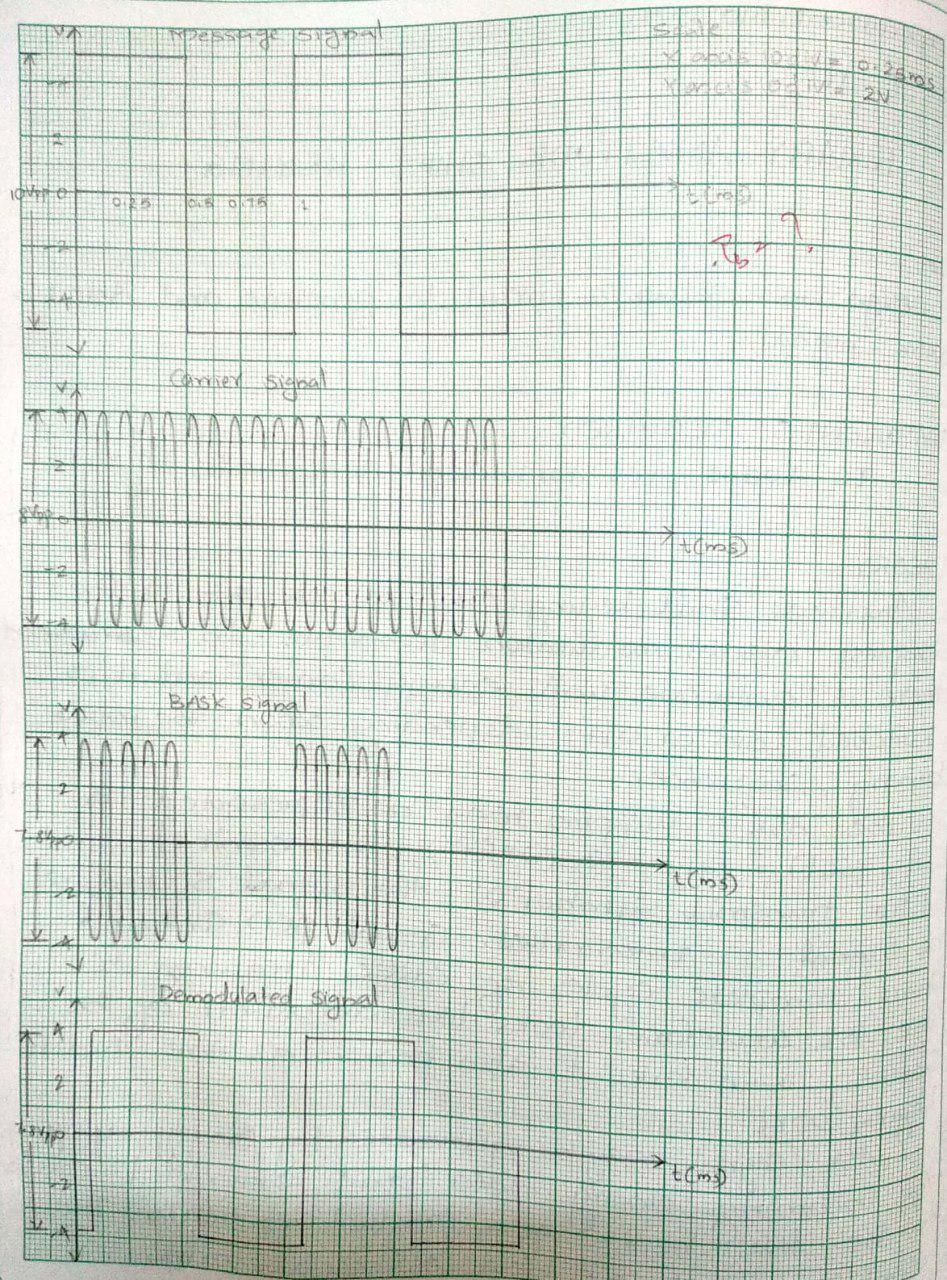
\includegraphics[width=0.6\textwidth]{bask-waveforms.jpg}
\caption{BASK waveforms}
\label{baskmod}
\end{figure}


\section*{Design}
\subsection*{BASK Generation}

BASK signal may be generated by simply applying the incoming binary data and sinusoidal carrier to the two inputs of an analog switch. When the binary data is applied to the control input of the switch, resulting output will be a BASK waveform. Ensure the carrier frequency is higher compared to the binary data frequency. 


\subsection*{BASK Demodulation}

Binary ASK signal can be demodulated non-coherantly using an envelop detector. This greatly simplifies the design cnsiderations required in synchronous detection. Non-coherant detection schemes  do not require a phase coherant local oscillator. 

\noindent Use 0A79 diode and $1 k\Omega $ resistor for rectification.
\noindent Use a simple RC lowpass filter to pass the low frequency binary message. Assuming the message frequecny is less than $1.5 kHz$,
 
\begin{equation}
f_H=\frac{1}{2\pi R_dC_d}
\end{equation}
\begin{equation}
1.5\ kHz=\frac{1}{2\pi R_dC_d}
\end{equation}
\noindent Select $C_d=\ 0.1 \mu F$. Then $R_d=\ 1k\Omega$.
Choose $R_d=\ 1k\Omega$ standard resistor value.\\

The resulting sequency may not be a perfect binary square wave. It can be transformed to a perfect binary sequence by using a threshold detector. The threshold level may adjusted using a $5 k\Omega$ pot.

\clearpage
\section*{Circuit Diagram}

The BASK generation using analog switching IC 4046 is shown in Figure \ref{bask-gen} and demodulation using envelop detection technique is shown in Figure \ref{bask-det}.

\begin{figure}
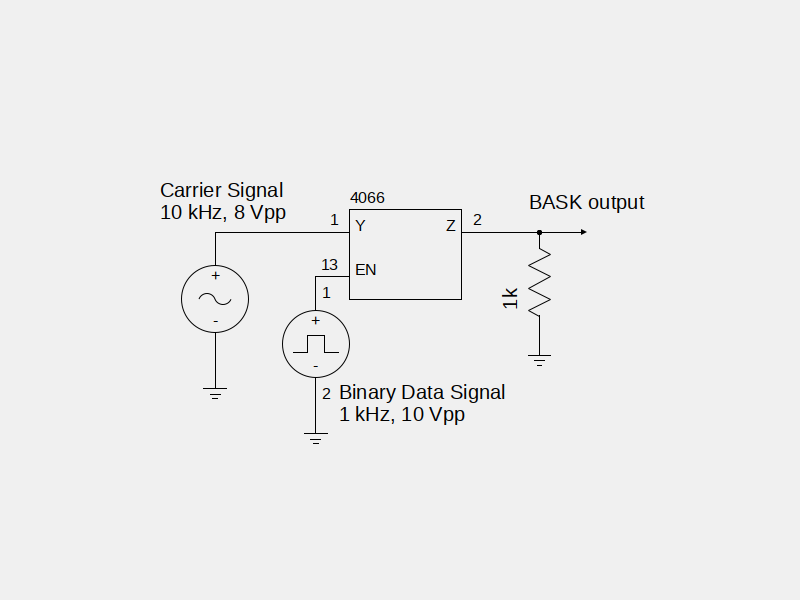
\includegraphics[width=0.8\textwidth]{bask.png}
\caption{BASK generation Circuit}
\label{bask-gen}
\end{figure}

\begin{figure}
	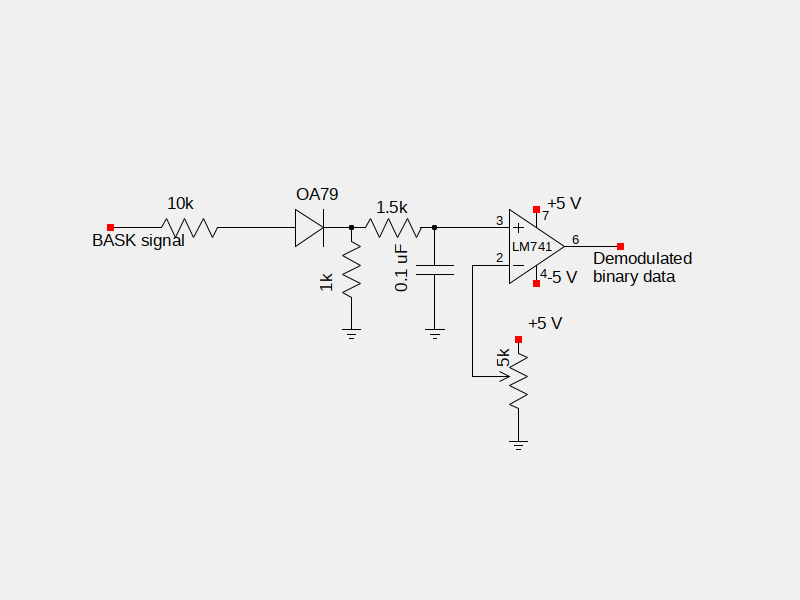
\includegraphics[width=0.8\textwidth]{bask-demod.png}
	\caption{BASK Demodulation Circuit}
	\label{bask-det}
\end{figure}


\section*{Procedure}
\begin{itemize}
\item
Connect the BASK generating circuit as shown in the circuit diagram, Figure \ref{bask-gen}.
\item
Feed the binary message data ($10 V_{pp}, 1 kHz$ square wave) and the carrier waveform  ($8 V_{pp}, 10 kHz$ sine wave) from the function generator.
\item
Observe the output on a CRO and plot the graphs of the input and output waveforms.
\item
Make the demodulating circuit as shown in the circuit diagram, Figure \ref{bask-det}.
\item
Observe the input and output waveforms from BASK demodulator.
\item 
Obtain the output of demodulator and the control input simultaneously, take the measurements and plot the waveforms.

\end{itemize}
\section*{Observation}
Plot the graphs of input and outout waveforms as observed on a CRO.
\section*{Result}

Implemented the PAM generation and demodulation circuits using BJT as well as switching IC.